%%% -*- TeX-master: "../main" -*-
\chapter{A Gesture Dataset}
\label{cha:gesture-dataset}

\citeauthor{murphy12} defines machine learning as \enquote{a set of methods that
  can automatically detect patterns in data, and then use the uncovered patterns
  to predict future data, or to perform other kinds of decision making under
  uncertainty} \cite{murphy12}. His definition underlines the central role of
data in learning and, consequently, the data corpus that we train our deep
models on will be of critical importance to their success. One of the important
insights of the deep learning revolution in computer vision was that you need
truly massive datasets to drive neural networks to peak performance. As a
result, research groups have amassed public datasets of visual imagery for
general purpose tasks as well as for specialized applications, including gesture
recognition. Given the high cost of creating neuromorphic datasets from scratch,
researchers have taken the logical next step and thought up a number of methods
to convert these image datasets into neuromorphic datasets. One possible way is
through simulation. \cite{barranco2016dataset} converted the Middlebury dataset
\cite{middlebury} by feeding a model of a neuromorphic camera with the image
data and the provided ground truth optical flow. Secondly, they also applied the
same methodology to purely synthetic data generated from a 3-dimensional virtual
world created in Blender. However, both of these methods produce insufficient
results when compared to actual DVS recordings because the type of noise
exhibited by the physical sensor is difficult to synthesize.
\cite{liu2016benchmarking} developed a method to convert large amounts of image
data into event data with realistic noise where they place a DVS in front of a
screen that either flashes an image repeatedly or moves it through the DVS's
field of view. Both kinds of presentation excite the DVS' pixels through
apparent motion, yet the generated data unsatisfactory. An object popping in and
out of existence is not representative of reality and their second idea has the
image moving in discrete steps, i.e. at least one pixel at a time, which
produces an unnatural distribution of events. A third and promising idea is
derived from a microscopic, twitching movement called a saccade that the human
eye performs up to a hundred times a second and which was found to be essential
to vision. \cite{orchard2015converting} recreate this mechanism by mounting a
DVS on a pan-tilt base and placing it in front of a screen showing images. The
apparatus then pans and tilts cyclically which stimulates the DVS's pixels
continuously as opposed to the discrete excitations from a moving image. After
careful consideration, we concluded that these approaches either produced
unsatisfactory results or required too much setup work and decided to record our
own dataset instead.

\citeauthor{tan2015benchmarking} analyzed computer vision datasets to deduce
guidelines for the neuromorphic vision community for creating useful datasets
\cite{tan2015benchmarking}. Their points most relevant to a dataset for this
thesis are, first, that a dataset should be representative of the real word and,
at the same time, a dataset should be challenging and just outside of the realm
of what is currently possible. A corpus that is too easy or clean to the point
where it can be solved with existing methods will be irrelevant because it does
not further the field. On the other hand, a data corpus that is too hard will
not be of any use because new ideas will fail on it regardless of their quality.
These arguments also preclude neuromorphic datasets derived from image datasets
in any of the ways above.

\begin{figure}[h]
  \centering
  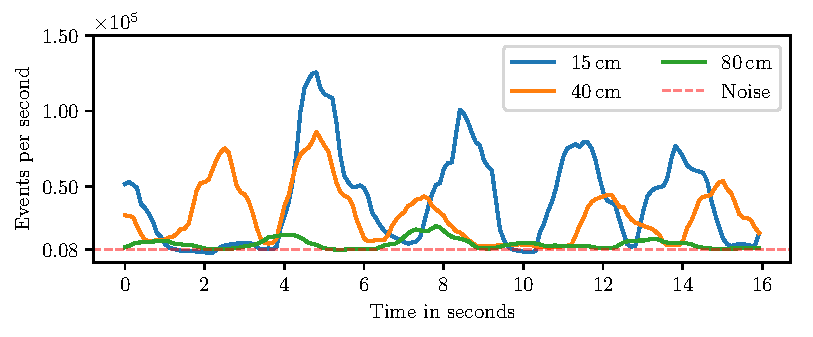
\includegraphics{figures/dataset/densities}
  \caption{Event density for various distances between the hand and the DVS}
  \label{fig:densities}
\end{figure}

We kept these guidelines in mind when we designed our dataset. Previous works on
neuromorphic gesture recognition worked with 3, 6 or 11 gestures, so we opted
for the 25 gestures that \cite{molchanov2016online} have used for recognition in
classical vision. They are listed in Table \ref{tab:gestures}. Our first dataset
consisted of 22 recordings of one subject with each gesture performed once in
each recording. To increase the variation, the subject wore different kinds of
clothing and varied the distance to the sensor between each recording. The kind
of clothing turned out to be an irrelevant factor because a resolution of
128$\times$128 is too coarse to make out such fine details. On the contrary, the
distance is a significant source of variation. Figure \ref{fig:densities} shows
the event rates of three recordings taken at three different distances. In tests
we have measured a noise event rate of about \SI{8}{keps} when the DVS is
directed towards a static scene which is the baseline rate between gestures
regardless of the distance. The peaks in the event rate show that the event rate
above baseline is proportional to the gap between hand and DVS because the main
source of events, the hand, takes up less space in the field of view of the
camera and stimulates fewer pixels. On the grounds that recordings with a gap
length of over \SI{60}{\centi\meter} were at times almost indistinguishable from
noise and it was even difficult for a human viewer to tell the gestures apart,
we had to exclude them from the dataset. Very close up recordings had to be
excluded for a different reason. They have a great signal-to-noise ratio, yet
the hand is so close to the sensor that it leaves the camera's field of view for
significant stretches of time during some gestures, and we were concerned that
this would render the gestures indistinguishable. All things considered, we
fixed the distance to about \SI{40}{} to \SI{50}{\centi\meter} and removed
recordings with significantly different gap lengths because that resulted in an
acceptable compromise between the two criteria. This reduced the size of the
25-gesture dataset to 18 recordings.

The complete set of 25 gestures listed in Table \ref{tab:gestures} proved
problematic nonetheless. We were concerned from the start because the corpus has
a high inter-class similarity and we had fewer examples per class than there
were classes. For example, \texttt{two-fingers-down} and \texttt{swipe-down} are
almost the same movement with the one difference that the former just uses two
fingers instead of four. Indeed, a first complete run through the recognition
system revealed these concerns to be justified as you can see in the confusion
matrix shown in Figure \ref{fig:confusion-25}. In this visualization, we
identified nine gestures that posed particular difficulties for our system.
These include all \texttt{two-fingers-*} classes as explained above,
\texttt{extend-*} because they are confused with a tapping motion,
\texttt{tap-two-fingers} because it is hard to distinguish between tapping with
a single or multiple fingers and finally \texttt{grab} because it is too similar
to \texttt{rotate-outward}.

\begin{figure}[h]
  \centering
  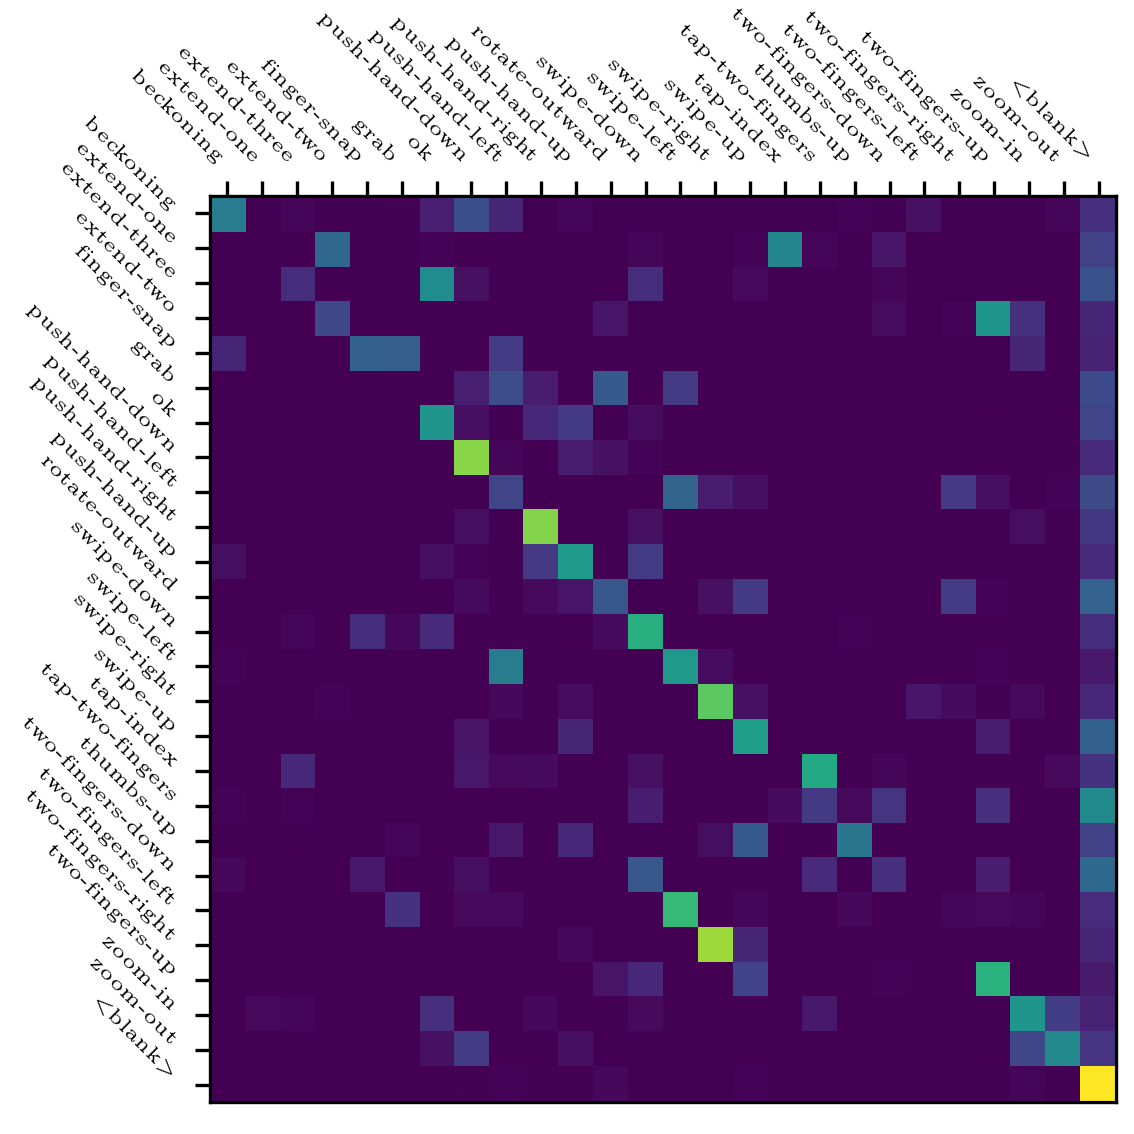
\includegraphics[width=4in]{figures/dataset/confusion-matrix}
  \caption{Confusion matrix for an initial run on the 25-gesture dataset}
  \label{fig:confusion-25}
\end{figure}

At that point, we chose to discard the 25-gesture corpus in favor of a new
dataset that would exclude the nine problematic gestures and at the same time
have more instances per class performed by more subjects. This second dataset
only includes the reduced set of gestures listed in the right-most column of
Table \ref{tab:gestures} which are performed by two subjects. Both subjects did
twenty recordings each of which contains all sixteen gestures in random order.
During the recording, the subject would position themselves so that they could
comfortably hold their right hand centrally in front of the DVS at a distance of
about \SI{50}{\centi\meter}. This time we did not make the subjects change their
appearance in any way between recordings. We also ensured constant illumination
by daylight because changing lighting conditions can create virtual edges and
therefore events on otherwise smooth surfaces when shadows move across them.

In the end, we collected two datasets, a small one with 25 gestures and a larger
one with 16 gestures. However, the first is only used in combination with the
latter on an unsupervised learning task described in Section
\ref{sec:autoencoder} because there the actual gestures are only secondary and
so we can cheaply profit from the additional data. For everything else, we rely
on the 16-gesture set only. We could have tried to reuse parts of the original
dataset since, after all, the remaining 16 gestures are a subset of the original
25. Yet we decided against it because the other classes are still present in the
data and both options of handling them are unsatisfactory. In a brute-force
approach, we could have deleted all events that belong to one of the excluded
classes, but that would have resulted in abrupt cuts in the recordings. Another
idea is to relabel these classes as one special \texttt{other} class, but that
class would necessarily be easy to mix up with all other classes.

Each recording is labeled in two ways. First, we have stored the so-called
recording log that states the random order in which the subject performed the
gestures and which is what we ultimately want the software to reconstruct from
the data. Second, we have segmented each recording explicitly with a
purpose-built software. In this case segmentation of a time series means a list
of start and end timestamps for each gesture. We have divided the dataset into a
training and a validation set where the last two recordings of each subject
constitute the validation set and the rest becomes the training set.

In Section \ref{sec:recording} we describe the software we developed for
recording and how it came to be. Section \ref{sec:segmentation} showcases the
software for segmenting the data. Finally, we describe the preprocessing of the
data in Section \ref{sec:preprocessing}.

\begin{table}
  \centering
  \begin{tabular}{c|c|c}
    % BEGIN RECEIVE ORGTBL gestures
Gesture & 25 dataset & 16 dataset\\
\hline
beckoning & \(\checkmark\) & \(\checkmark\)\\
extend-one & \(\checkmark\) & \\
extend-three & \(\checkmark\) & \\
extend-two & \(\checkmark\) & \\
finger-snap & \(\checkmark\) & \(\checkmark\)\\
grab & \(\checkmark\) & \\
ok & \(\checkmark\) & \(\checkmark\)\\
push-hand-down & \(\checkmark\) & \(\checkmark\)\\
push-hand-left & \(\checkmark\) & \(\checkmark\)\\
push-hand-right & \(\checkmark\) & \(\checkmark\)\\
push-hand-up & \(\checkmark\) & \(\checkmark\)\\
rotate-outward & \(\checkmark\) & \(\checkmark\)\\
swipe-down & \(\checkmark\) & \(\checkmark\)\\
swipe-left & \(\checkmark\) & \(\checkmark\)\\
swipe-right & \(\checkmark\) & \(\checkmark\)\\
swipe-up & \(\checkmark\) & \(\checkmark\)\\
tap-index & \(\checkmark\) & \(\checkmark\)\\
tap-two-fingers & \(\checkmark\) & \\
thumbs-up & \(\checkmark\) & \(\checkmark\)\\
two-fingers-down & \(\checkmark\) & \\
two-fingers-left & \(\checkmark\) & \\
two-fingers-right & \(\checkmark\) & \\
two-fingers-up & \(\checkmark\) & \\
zoom-in & \(\checkmark\) & \(\checkmark\)\\
zoom-out & \(\checkmark\) & \(\checkmark\)\\
    % END RECEIVE ORGTBL gestures
  \end{tabular}
  \caption{List of gestures in the datasets}
  \label{tab:gestures}
\end{table}
\begin{comment}
  #+ORGTBL: SEND gestures orgtbl-to-latex :splice t
  | Gesture           | 25 dataset | 16 dataset |
  |-------------------+------------+------------|
  | beckoning         | \checkmark | \checkmark |
  | extend-one        | \checkmark |            |
  | extend-three      | \checkmark |            |
  | extend-two        | \checkmark |            |
  | finger-snap       | \checkmark | \checkmark |
  | grab              | \checkmark |            |
  | ok                | \checkmark | \checkmark |
  | push-hand-down    | \checkmark | \checkmark |
  | push-hand-left    | \checkmark | \checkmark |
  | push-hand-right   | \checkmark | \checkmark |
  | push-hand-up      | \checkmark | \checkmark |
  | rotate-outward    | \checkmark | \checkmark |
  | swipe-down        | \checkmark | \checkmark |
  | swipe-left        | \checkmark | \checkmark |
  | swipe-right       | \checkmark | \checkmark |
  | swipe-up          | \checkmark | \checkmark |
  | tap-index         | \checkmark | \checkmark |
  | tap-two-fingers   | \checkmark |            |
  | thumbs-up         | \checkmark | \checkmark |
  | two-fingers-down  | \checkmark |            |
  | two-fingers-left  | \checkmark |            |
  | two-fingers-right | \checkmark |            |
  | two-fingers-up    | \checkmark |            |
  | zoom-in           | \checkmark | \checkmark |
  | zoom-out          | \checkmark | \checkmark |
\end{comment}

\section{Recording Software}
\label{sec:recording}

Our dataset consists of a number of recordings, each of which shows a subject
performing each gesture exactly once in random order. In a first attempt, we
planned on combining all aspects into one program with the intention of making
the experience a smooth one for the subject and time-saving for the instructor.
So we wrote a program called \texttt{recorder} that was meant to show
instructional videos to the subject, instruct them on when to perform a gesture
with a countdown and in which order and would also let the instructor segment
the time series at the same time. After a first iteration, we saw that we had
failed by all accounts. The program was unstable, probably due to the direct
device access with a C library, and crashed from time to time, the countdown
made the experience unnecessarily stressful for the subject and the
segmentations were inaccurate because each subject has their own rhythm in
performing when the countdown hits zero. Because of these shortcomings, we
scrapped \texttt{recorder} and split its functionality into separate programs
with well-separated responsibilities.

\begin{figure}[h]
  \centering
  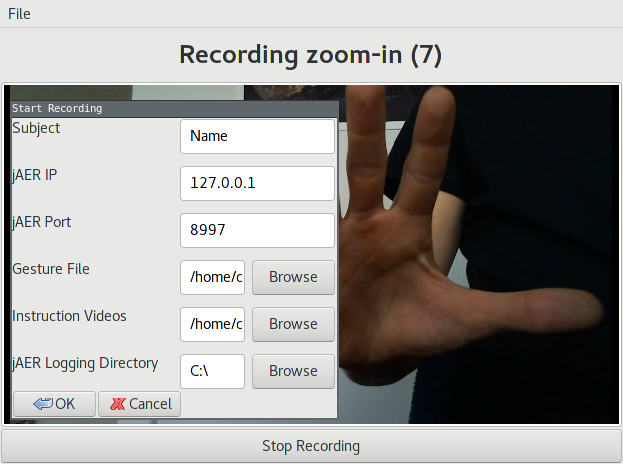
\includegraphics{figures/dataset/jaerrec}
  \caption{User interface of \texttt{jaerrec}}
  \label{fig:jaerrec}
\end{figure}

The successor is called \texttt{jaerrec} and you can see its user interface in
Figure \ref{fig:jaerrec}. On the left is the setup dialog for a recording and in
the background is the instruction video for \texttt{zoom-in}. The recording of
the event stream is offloaded to jAER which \texttt{jaerrec} controls remotely
via UDP commands. This leaves it with the responsibility of playing the
instruction videos in the order provided by the recording log that is generated
beforehand and is just a random permutation of all gestures. Due to the stress
induced by the timing requirements and the resulting inaccuracy the
semi-automatic segmentation, we split that part off into a separate program as
well.

\section{Segmentation Software}
\label{sec:segmentation}

\begin{figure}
  \centering
  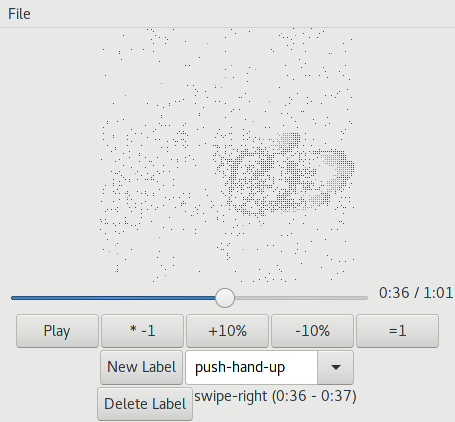
\includegraphics{figures/dataset/labeler.png}
  \caption{User interface of \texttt{labeler}}
  \label{fig:labeler}
\end{figure}

We have written an extra labeling software called \texttt{labeler} shown in
Figure \ref{fig:labeler} that is optimized to minimize the time it takes to
segment a recording while giving the user the tools to place the gesture
boundaries with high precision. It reads the recording log of gestures together
with the recorded data and replays it. Then the user guides the segmentation
process with just the ``New Label''. The process is implemented as a
finite-state machine with three states and only a single transition going in and
out of each state. The default state is \texttt{looking-for-gesture} where the
playback happens at 150\% to quickly skip irrelevant time between gestures. When
the user spots a gesture, he or she clicks the button and the machine
transitions to a new state \texttt{looking-for-start}. In that state the
playback runs in reverse at 50\% speed so that the user can place the start
marker accurately. When he has spotted the beginning of the gesture, he or she
clicks again which marks the start and transitions to the last state
\texttt{looking-for-end}. Now the playback reverses again though it is still
slowed down. One last click at the end of the gesture adds the start and end
markers to the segmentation and transitions back to the initial state. The name
of the gesture is automatically taken from the recording log by keeping a count
of how many gestures have been marked already. This optimized process reduces
the user interaction in the general case to the repeated clicking of a single
button and allows the segmentation of one minute of recorded material in about
three minutes. Figure \ref{fig:segmentation} showcases a finished segmentation.

\begin{figure}
  \centering
  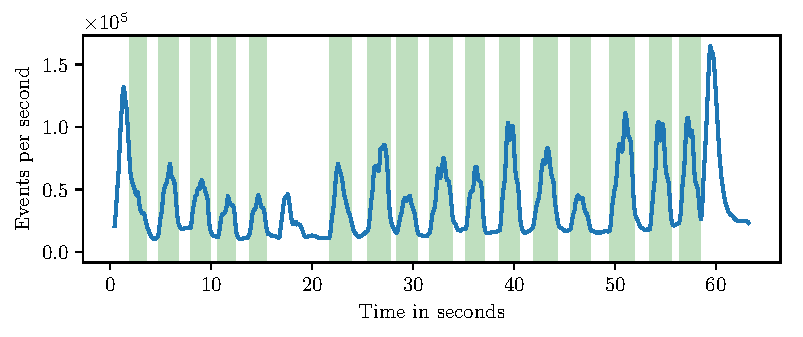
\includegraphics{figures/dataset/segmentation}
  \caption{A segmentation created with \texttt{labeler}. The line plots the
    event density and the shaded regions mark the extent of the gestures.}
  \label{fig:segmentation}
\end{figure}

\section{Preprocessing}
\label{sec:preprocessing}

Figure \ref{fig:heatmap} shows a heatmap of all events in a recording and it
looks about as expected. In the left half one can barely make out the outline of
the subject, but most events are clustered in the center where the subject held
his or her hand. Near the top are two outliers, colored yellow and green, that
are significantly brighter than any pixel in their neighborhood. These are most
likely faulty circuits that trigger continuously. On the other hand, a handful
of pixels in the top right did not generate a single event over the course of
this recording and are most likely faulty as well.

\begin{figure}[h]
  \centering
  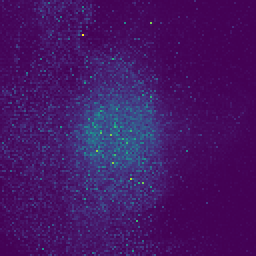
\includegraphics[width=2in]{figures/dataset/heatmap}
  \caption{Heatmap of pixel activity}
  \label{fig:heatmap}
\end{figure}

Even though the data has the expected form, it is still unfit for further
processing for several reasons. First, the timestamps of the events are steadily
increasing which means that the event sequence is not time-invariant, i.e. the
same gesture performed a second later would generate a different sequence.
Second, the time series is not location-invariant because the $x$ and $y$
coordinates are absolute with respect to the origin. This means that a gesture
performed in the bottom-left corner of the field of view would produce a time
series different from the identical gesture performed near the center. Last, the
data is not standardized. Most machine learning algorithms, including deep
learning, perform best when the features have mean $0$ and standard deviation
$1$.

We made the event sequence time-invariant by introducing a new feature $\delta
t$ that is defined as the time passed since the previous event, i.e. $\delta
t^{(i)} = t^{(i)} - t^{(i - 1)}$ with a value of $0$ as the base case. In this
way, we have replaced an absolute point of reference, some arbitrary point in
time, with a point of reference that is defined by the data itself, in this case
simply the timestamp of the previous event. To make the data location-invariant
we need to introduce a relative reference point for $x$ and $y$ as well. Assume
that we would have gone with the same naive idea as we did for $t$. Then an
actual event following a noise event would also receive random nonsense values
for $\delta x$ and $\delta y$ just as the noise event did, effectively doubling
the amount of noise in the data. Therefore, this line of thought necessitated a
more stable point of reference. Our solution is to keep track of a mean with
exponentially decaying weights because it gives more weight to recent events and
can be cheaply computed in a streaming context such as online recognition. Such
a mean $\mu_{x}$ that tracks a quantity $x$ through continuous time is defined
as
\begin{equation*}
  \mu_{x}^{(i)} = \left( 1 - \alpha^{t^{(i)} - t^{(i - 1)}} \right) \cdot x^{(i)} + \alpha^{t^{(i)} - t^{(i - 1)}} \cdot \mu_{x}^{(i - 1)}
\end{equation*}
where $x^{(i)}$ was observed at time $t^{(i)}$. The parameter $\alpha$ controls
how much weight is placed in past data. The extreme cases of $\alpha = 0$ and
$\alpha = 1$ do not keep track of history at all respectively never change
$\mu_{x}$ from its initial value. To make this parameter $\alpha$ more
meaningful, we use the half-life reparameterization with the parameter
$\lambda$. When you plug in the following
\begin{equation*}
  \alpha = \exp\left( \frac{\log\left( \frac{1}{2} \right)}{\lambda} \right),
\end{equation*}
all values of $x^{(i)}$ that were observed more than $\lambda$ time ago are
assigned a total weight of one half.

We then keep two means for each of $x$ and $y$, one with $\lambda = \SI{1}{s}$
and another with $\lambda = \SI{50}{\milli\second}$. The first is supposed to
track the main movement of the hand, while we intend the second to track fast
movement like individual fingers. Figure \ref{fig:ewm-means} plots both means
for the $x$-coordinate and shows that the intended effect was achieved. For
example, the third shaded region in that plot marks a \texttt{swipe-right}
gesture where the subject first moves the hand slightly left and then in a wavy
motion to the right.

\begin{figure}[h]
  \centering
  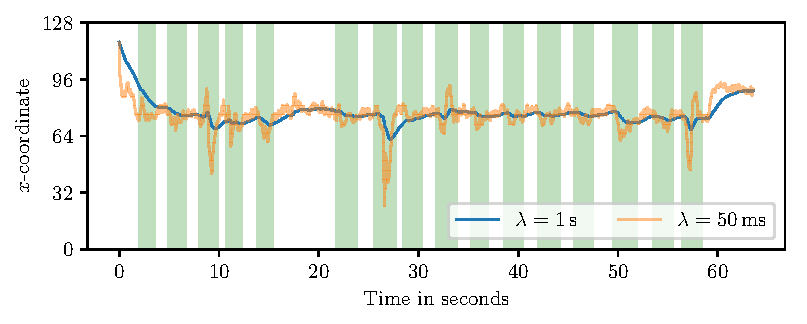
\includegraphics{figures/dataset/ewm-means}
  \caption{Slow and fast tracking means of the $x$ coordinate of an event stream}
  \label{fig:ewm-means}
\end{figure}

On the whole the preprocessing maps each event from four features to six
features as follows
\begin{equation*}
  \left( t^{(i)}, x^{(i)}, y^{(i)}, p^{(i)} \right) \mapsto \left( \delta t^{(i)}, \delta x_{\lambda = \SI{1}{\second}}^{(i)}, \delta x_{\lambda = \SI{50}{\milli\second}}^{(i)}, \delta y_{\lambda = \SI{1}{\second}}^{(i)}, \delta y_{\lambda = \SI{50}{\milli\second}}^{(i)}, p^{(i)} \right)
\end{equation*}
where $\delta x_{\lambda = \SI{1}{\second}}^{(i)} = x^{(i)} -
\mu_{x,\lambda=\SI{1}{\second}}^{(i)}$ et cetera. None of the final features has
an absolute point of reference, so they are time- as well as location-invariant.

Finally, we need to standardize the attributes. Let $X \subset \mathbb{R}^{6}$
be a set of preprocessed events. Then we compute the sample mean $\mu_{X}$ and
standard deviation $\sigma_{X}$ by
\begin{equation*}
  \mu_{X} = \frac{1}{|X|} \sum_{x \in X} x \quad \textrm{and} \quad \sigma_{X} = \sqrt{\frac{1}{|X|} \sum_{x \in X} \left( x - \mu_{X} \right)^{2}}
\end{equation*}
where the squaring and square-root are applied component-wise. Then we replace
each $x_{i}$ by $\bar{x}_{i} = \frac{x_{i} - \mu_{X}}{\sigma_{X}}$ where the
division again is done component-wise. Note that we also standardize the
polarity because OFF events outnumber ON events about 60/40, so its mean and
standard deviation are not quite $0$ and $1$, respectively. This final set
$\bar{X}$ then constitutes a fully preprocessed training set. Of course, the
sample $\mu$ and $\sigma$ are reused from the training set to preprocess the
validation and test sets.

At the time, when we designed this process, we were also worried about
scale-invariance. The effect of scale is nicely shown in Figure
\ref{fig:densities}. In that plot we can see that the event rate depends
directly on the distance between the subject and the DVS. So the same gesture
performed up close to and bit farther from the sensor would still result in very
different recordings. Accounting for this would entail accounting for spatial as
well as temporal scale because events from a close-up gesture are spread further
across the DVS's field of view as well as take up longer stretches in the event
stream. We have experimented with normalizing the data in both regards. We
estimated the spatial extent of a gesture with a Kalman filter and scaled the
event coordinates proportional to that measure. Regarding the higher event rate,
we subsampled the data down to a target event rate. In the end, we decided that
our measures regarding scale-invariance were not effective enough and fixed the
distance between subject and sensor instead.

Table \ref{tab:dataset-stats} lists statistics about the final dataset. The
first thing to note is that not every gesture was performed exactly 40 times as
one would expect from two subjects repeating each gesture 20 times. Instead some
gestures were performed twice to make sure that they were clearly visible. The
average duration of a gesture is between 1.3 and 2 seconds with only a small
amount of variation between each instance. However, the average number of events
per instance varies considerably between the classes and also between iterations
of the same gesture as testified by the large ratio between the means and
standard deviations. The data not belonging to any class, labelled
\texttt{<blank>}, makes up about half of the data measured in seconds yet it is
only 29\% of the event data. This is due to the reduced event rate between
gestures when the subject's movement is minimal.

\begin{table}
  \centering
  \begin{tabular}{r|c|l|l}
    % BEGIN RECEIVE ORGTBL stats
Gesture & \# & Time & Events\\
\hline
beckoning & 41 & \SI{67}{\second} (\(\mu = \SI{1.6}{\second}, \sigma = \SI{0.2}{\second}\)) & 2,949,776 (\(\mu = 71,945, \sigma = 29,515\))\\
finger-snap & 40 & \SI{59}{\second} (\(\mu = \SI{1.5}{\second}, \sigma = \SI{0.3}{\second}\)) & 2,203,881 (\(\mu = 55,097, \sigma = 19,777\))\\
ok & 40 & \SI{63}{\second} (\(\mu = \SI{1.6}{\second}, \sigma = \SI{0.2}{\second}\)) & 3,054,306 (\(\mu = 76,357, \sigma = 18,290\))\\
push-hand-down & 41 & \SI{77}{\second} (\(\mu = \SI{1.9}{\second}, \sigma = \SI{0.3}{\second}\)) & 4,000,518 (\(\mu = 97,573, \sigma = 33,154\))\\
push-hand-left & 40 & \SI{74}{\second} (\(\mu = \SI{1.9}{\second}, \sigma = \SI{0.4}{\second}\)) & 3,859,846 (\(\mu = 96,496, \sigma = 32,781\))\\
push-hand-right & 39 & \SI{76}{\second} (\(\mu = \SI{1.9}{\second}, \sigma = \SI{0.3}{\second}\)) & 5,550,913 (\(\mu = 142,331, \sigma = 57,933\))\\
push-hand-up & 41 & \SI{84}{\second} (\(\mu = \SI{2.0}{\second}, \sigma = \SI{0.3}{\second}\)) & 5,278,815 (\(\mu = 128,751, \sigma = 48,901\))\\
rotate-outward & 40 & \SI{51}{\second} (\(\mu = \SI{1.3}{\second}, \sigma = \SI{0.2}{\second}\)) & 2,104,242 (\(\mu = 52,606, \sigma = 18,325\))\\
swipe-down & 41 & \SI{68}{\second} (\(\mu = \SI{1.6}{\second}, \sigma = \SI{0.3}{\second}\)) & 3,789,590 (\(\mu = 92,429, \sigma = 47,715\))\\
swipe-left & 41 & \SI{66}{\second} (\(\mu = \SI{1.6}{\second}, \sigma = \SI{0.3}{\second}\)) & 3,709,310 (\(\mu = 90,470, \sigma = 36,633\))\\
swipe-right & 40 & \SI{65}{\second} (\(\mu = \SI{1.6}{\second}, \sigma = \SI{0.3}{\second}\)) & 3,339,538 (\(\mu = 83,488, \sigma = 39,184\))\\
swipe-up & 42 & \SI{71}{\second} (\(\mu = \SI{1.7}{\second}, \sigma = \SI{0.3}{\second}\)) & 4,359,013 (\(\mu = 103,786, \sigma = 38,998\))\\
tap-index & 40 & \SI{62}{\second} (\(\mu = \SI{1.6}{\second}, \sigma = \SI{0.2}{\second}\)) & 2,620,666 (\(\mu = 65,516, \sigma = 20,536\))\\
thumbs-up & 40 & \SI{55}{\second} (\(\mu = \SI{1.4}{\second}, \sigma = \SI{0.2}{\second}\)) & 1,939,608 (\(\mu = 48,490, \sigma = 15,750\))\\
zoom-in & 40 & \SI{73}{\second} (\(\mu = \SI{1.8}{\second}, \sigma = \SI{0.3}{\second}\)) & 3,414,950 (\(\mu = 85,373, \sigma = 36,047\))\\
zoom-out & 41 & \SI{74}{\second} (\(\mu = \SI{1.8}{\second}, \sigma = \SI{0.3}{\second}\)) & 3,425,209 (\(\mu = 83,541, \sigma = 28,812\))\\
<blank> & - & \SI{22.18}{\minute} & 28,865,096\\
\hline
Total & 647 & \SI{40.25}{\minute} & 84,465,277\\
    % END RECEIVE ORGTBL stats
  \end{tabular}
  \caption{Number of instances, total amount of data in seconds and number of
    events for each of the 16 gestures in the final dataset. The quantities in
    parentheses give the average per instance and the standard deviation.}
  \label{tab:dataset-stats}
\end{table}
\begin{comment}
  #+ORGTBL: SEND stats orgtbl-to-latex :splice t
  | Gesture         |   # | Time                                                                     | Events                                       |
  |-----------------+-----+--------------------------------------------------------------------------+----------------------------------------------|
  | beckoning       |  41 | \SI{67}{\second} ($\mu = \SI{1.6}{\second}, \sigma = \SI{0.2}{\second}$) | 2,949,776 ($\mu = 71,945, \sigma = 29,515$)  |
  | finger-snap     |  40 | \SI{59}{\second} ($\mu = \SI{1.5}{\second}, \sigma = \SI{0.3}{\second}$) | 2,203,881 ($\mu = 55,097, \sigma = 19,777$)  |
  | ok              |  40 | \SI{63}{\second} ($\mu = \SI{1.6}{\second}, \sigma = \SI{0.2}{\second}$) | 3,054,306 ($\mu = 76,357, \sigma = 18,290$)  |
  | push-hand-down  |  41 | \SI{77}{\second} ($\mu = \SI{1.9}{\second}, \sigma = \SI{0.3}{\second}$) | 4,000,518 ($\mu = 97,573, \sigma = 33,154$)  |
  | push-hand-left  |  40 | \SI{74}{\second} ($\mu = \SI{1.9}{\second}, \sigma = \SI{0.4}{\second}$) | 3,859,846 ($\mu = 96,496, \sigma = 32,781$)  |
  | push-hand-right |  39 | \SI{76}{\second} ($\mu = \SI{1.9}{\second}, \sigma = \SI{0.3}{\second}$) | 5,550,913 ($\mu = 142,331, \sigma = 57,933$) |
  | push-hand-up    |  41 | \SI{84}{\second} ($\mu = \SI{2.0}{\second}, \sigma = \SI{0.3}{\second}$) | 5,278,815 ($\mu = 128,751, \sigma = 48,901$) |
  | rotate-outward  |  40 | \SI{51}{\second} ($\mu = \SI{1.3}{\second}, \sigma = \SI{0.2}{\second}$) | 2,104,242 ($\mu = 52,606, \sigma = 18,325$)  |
  | swipe-down      |  41 | \SI{68}{\second} ($\mu = \SI{1.6}{\second}, \sigma = \SI{0.3}{\second}$) | 3,789,590 ($\mu = 92,429, \sigma = 47,715$)  |
  | swipe-left      |  41 | \SI{66}{\second} ($\mu = \SI{1.6}{\second}, \sigma = \SI{0.3}{\second}$) | 3,709,310 ($\mu = 90,470, \sigma = 36,633$)  |
  | swipe-right     |  40 | \SI{65}{\second} ($\mu = \SI{1.6}{\second}, \sigma = \SI{0.3}{\second}$) | 3,339,538 ($\mu = 83,488, \sigma = 39,184$)  |
  | swipe-up        |  42 | \SI{71}{\second} ($\mu = \SI{1.7}{\second}, \sigma = \SI{0.3}{\second}$) | 4,359,013 ($\mu = 103,786, \sigma = 38,998$) |
  | tap-index       |  40 | \SI{62}{\second} ($\mu = \SI{1.6}{\second}, \sigma = \SI{0.2}{\second}$) | 2,620,666 ($\mu = 65,516, \sigma = 20,536$)  |
  | thumbs-up       |  40 | \SI{55}{\second} ($\mu = \SI{1.4}{\second}, \sigma = \SI{0.2}{\second}$) | 1,939,608 ($\mu = 48,490, \sigma = 15,750$)  |
  | zoom-in         |  40 | \SI{73}{\second} ($\mu = \SI{1.8}{\second}, \sigma = \SI{0.3}{\second}$) | 3,414,950 ($\mu = 85,373, \sigma = 36,047$)  |
  | zoom-out        |  41 | \SI{74}{\second} ($\mu = \SI{1.8}{\second}, \sigma = \SI{0.3}{\second}$) | 3,425,209 ($\mu = 83,541, \sigma = 28,812$)  |
  | <blank>         |   - | \SI{22.18}{\minute}                                                      | 28,865,096                                   |
  |-----------------+-----+--------------------------------------------------------------------------+----------------------------------------------|
  | Total           | 647 | \SI{40.25}{\minute}                                                      | 84,465,277                                   |
\end{comment}
